\newsavebox{\boxcc}
\Savebox{\boxcc}{
\hspace{-0.25cm}
\begin{minipage}[l]{\columnwidth}
\begin{lstlisting}[style=conescframe]
context group BaseStationG {
*\lstnote{layereddef}* layered command void report(msg_t msg);
}implementation {
*\lstnote{contexts}* contexts Reachable,
*\lstnote{isdefault}*          Unreachable is default,
*\lstnote{iserror}*          MyErrorC is error;
 components Routing, Logging;
 Reachable.Collection -> Routing;
 Unreachable.DataStore -> Logging;}
\end{lstlisting}
\end{minipage}
}
\newsavebox{\boxbscm}
\Savebox{\boxbscm}{
\hspace{-0.25cm}
\begin{minipage}[l]{\columnwidth}
\begin{lstlisting}[style=conescframe]
module BaseStationContextManager {
 uses context group BaseStationG;
}implementation {
 event msg_t Beacon.receive(msg_t msg) {
*\lstnote{actBS}*  activate BaseStationG.Reachable;
  call BSReset.stop(); 
  call BSReset.startOneShot(TIMEOUT);}
 event void BSReset.fired() {
*\lstnote{actNoBS}*  activate BaseStationG.Unreachable;}}
\end{lstlisting}
\end{minipage}
}
\newsavebox{\boxc}
\Savebox{\boxc}{
\hspace{-0.25cm}
\begin{minipage}[l]{\columnwidth}
\begin{lstlisting}[style=conescframe]
context Unreachable {
*\lstnote{dependence}* transitions Reachable iff ActivityG.Running;
 uses interface DataStore;
}implementation {
*\lstnote{activatedUnreachable}* event void activated(){//...}
*\lstnote{deactivatedUnreachable}* event void deactivated(){//...}
*\lstnote{checkUnreachable}* command bool check(){//...}
 layered command void report(msg_t msg){
*\lstnote{layeredimp}*  call DataStore.deposit(msg);}}
\end{lstlisting}
\end{minipage}
}
\newsavebox{\boxirc}
\Savebox{\boxirc}{
\hspace{-0.25cm}
\begin{minipage}[l]{\columnwidth}
\begin{lstlisting}[style=conescframe]
context Reachable {
 uses interface Collection;
 uses context group BatteryG; 
}implementation {
*\lstnote{activated}* event void activated(){ 
  call GPS.stop();}
*\lstnote{deactivated}* event void deactivated(){//...}
*\lstnote{check}* command bool check(){
  return call BatteryG.getContext() == BatteryG.Normal;}
 layered command void report(msg_t msg){
*\lstnote{layeredimp2}*  call Collection.send(msg);}}
\end{lstlisting}
\end{minipage}
}
\newsavebox{\boxlc}
\Savebox{\boxlc}{
\hspace{-0.25cm}
\begin{minipage}[l]{\columnwidth}
\begin{lstlisting}[style=conescframe]
context Low {
*\lstnote{triggers}* triggers BaseStationG.Unreachable;
}implementation {//...}
\end{lstlisting}
\end{minipage}
}
% \newsavebox{\boxmc}
% \Savebox{\boxmc}{
% \hspace{-0.25cm}
% \begin{minipage}[l]{\columnwidth}
% \begin{lstlisting}[style=conescframe]
% configuration ApplicationC {
% }implementation {
% *\lstnote{declaration}* components BaseStationG, Application;
%  //...
% *\lstnote{wiring}* Application.BaseStationG -> BaseStationG;}
% \end{lstlisting}
% \end{minipage}
% }
\newsavebox{\boxmm}
\Savebox{\boxmm}{
\hspace{-0.25cm}
\begin{minipage}[l]{\columnwidth}
\begin{lstlisting}[style=conescframe]
module User {
*\lstnote{cgdecl}* uses context group BaseStationG;
}implementation {
 event void Timer.fired() {
*\lstnote{calling}*  call BaseStationG.report(msg);}
*\lstnote{eventCC}* event void BaseStationG.contextChanged(context_t con) {
*\lstnote{concheck}*  if(con == BaseStationG.Reachable) // DO SOMETHING...}}
\end{lstlisting}
\end{minipage}
}
\newsavebox{\boxnmc}
\Savebox{\boxnmc}{
\hspace{-0.25cm}
\begin{minipage}[l]{\columnwidth}
\begin{lstlisting}[style=conescframe]
context NotMoving {
*\lstnote{transitions}* transitions Resting;
}implementation {//...}
\end{lstlisting}
\end{minipage}
}
\vspace{-0.09in}
\section{Context Oriented nesC (ConesC)} 

The main benefit of ConesC is a possibility to alternate the behavior of a software at
run-time. It implies also a run-time errors catching and handling. Our approach
provides a deep modularization as well. Thus, behavioral variations are encapsulated
into different modules. The latter, as we show in Sec.~\ref{sec:evalcomp},
are highly decoupled, which enhances code readability and re-usability as well as debugging
and developing processes. The behavioral variation can be achieved by calling a
layered function, since the contextual dependent logic is encapsulated by an isolated module, or
by catching and handling an error event, which can be invoked at run-time.

Programming in ConesC is tightly coupled with environment-dependent behavior of
the application and exploits two main concepts: \emph{i)} individual contexts
and their transitions and \emph{ii)} context groups. The former represent
different environment situations where a system may find itself. Each context
maps to a separate state of the device or environment a system operates in. As
the environment conditions change, a programmer initiates a context transition
by \emph{activating} the corresponding context. A context group is a set of contexts
sharing common characteristics. Thus, whenever a transition between involved
contexts occurs, it is determined by changes in one or more physical quantities.

\subsection{Application design}

The diagram on Fig.~\ref{fig:wtd} shows how these concepts are used in application's design.
Depending on GPS readings developers may want to vary a sampling rate to use energy
more effective. For example, there is no need to
track a location if an animal is \emph{Not Moving}, but should accelerometer detect any
significant movement, a periodic sampling should be initiated. Increased
difference between two location readings indicates that an animal is
\emph{Running}, and location sampling should occurs more often.
Here contexts~\emph{Running}, \emph{Resting} and~\emph{Not Moving} are based on
a physical quantity -- the velocity of an animal -- and reflect
variations of the same functionality, such as GPS sampling with a given frequency,
so they can be joined into a group.

In social networks there exists a motion~\cite{pasztor10}, which can be exploited to
reduce energy consumption. For example, it makes no sense to send beacons
from the node, which is attached to the most active animal in a herd, i.e.~\emph{Leader},
since the node communicates with the most nodes in the network. Opposite to~\emph{Leader},
other nodes send beacons to reveal themselves.

Orthogonal to application-level functionality, the system should transmit data to
the Base Station (BS) or save readings locally depending on the BS
availability. While the BS is \emph{Out Range}, GPS-sensor is used to
obtain the location and data is written in internal memory. But should the node
receive a BS-beacon, the data is dumped to the BS and GPS-sensor is disabled
since the location of the is well-known BS. The application also should be aware
of battery status and disable power consuming modules like GPS and GPRS if the
battery level is \emph{Low}.

ConesC reflects this design by using new types of components, such as
\emph{context} and \emph{context group}, which are extensions of \emph{module} and
\emph{configuration} correspondingly, and a set of new key-words.
Instances of new types, however, can also be used as standard nesC components,
e.g. they can provide or use interfaces as well as be declared in the same way.

\putfigure{caption=Wildlife tracking diagram.,label=fig:wtd}{
 \centering
 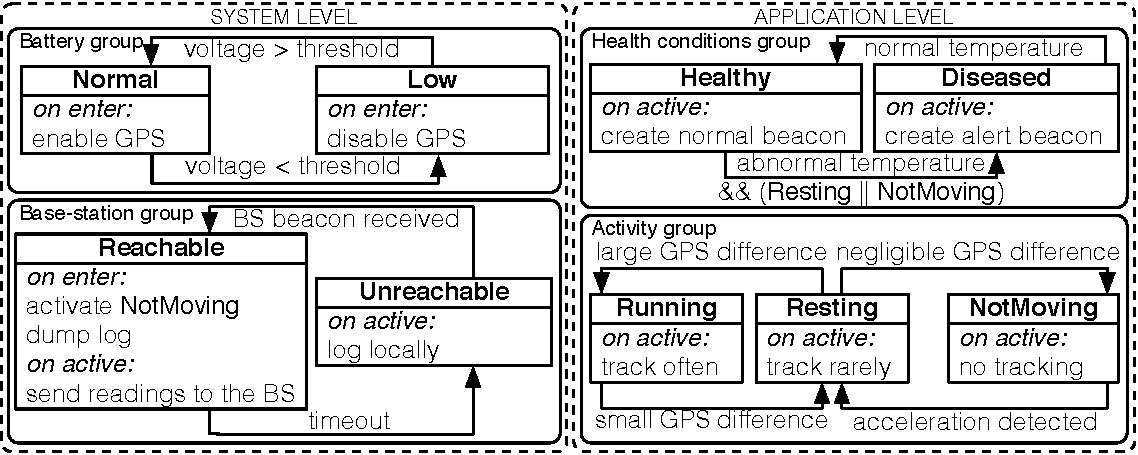
\includegraphics[width=\columnwidth]{pdf/wildlifetracking}
}

\subsection{Contexts and Context Groups}\label{subsec:components}

A \emph{Context group} component is displayed on Fig.~\ref{fig:ccc} and used to declare layered
functions as well as the included contexts. The former is declared on the line~\lstref{layereddef}
by using the key-word~\emph{layered}, while the declaration of the latter starts from the
key-word~\emph{contexts} on the line~\lstref{contexts}. It is mandatory to declare
the~\emph{default} context, as shown on the line~\lstref{isdefault}, which will be
activated at the beginning of the execution. The next line~\lstref{iserror} declares the
context~\emph{Error} as an~\emph{error} context, which is used to handle errors occurred
during the execution. If an~\emph{error} context is not declared, it will be generated automatically.
We discuss the use of this context in section~\ref{subsec:rules}.

\putsnippet{
 caption=Context configuration component.,
 label=fig:ccc,
 boxname=boxcc
}

Figures~\ref{fig:cc} and~\ref{fig:irc} displays a~\emph{Context} component, main
purpose of which is an implementation of layered function declared in context configuration. 
This approach enables a behavioral variation, since the implementation of a layered function is
context-specific, and only one context within the group can be active at a time. Thus, in our
example, a behavior of the function~\emph{report()} depends on the activated context and
deposits a message in local memory, while \emph{Out Range} context
is active (figure~\ref{fig:cc}, line~\lstref{layeredimp}),
or sends it directly to the BS otherwise (figure~\ref{fig:irc}, line~\lstref{layeredimp2}).
Programmer may want to add some instructions after
context activation such as initialization of variables or enabling/disabling
modules, as in our example in Fig.~\ref{fig:wtd} we enable GPS-sensor on entering
in~\emph{Out Range} context. Or it may be necessary to reset component's state before context
deactivation. To this end ConesC provides events \emph{activated()} and
\emph{deactivated()} correspondingly, whose stub implementation is shown on
lines~\lstref{activated} and~\lstref{deactivated} in Fig.~\ref{fig:cc}. The implementation of
these events, however, is not obligatory.

\putsnippet{
 caption=Context component.,
 label=fig:cc,
 boxname=boxc
}

\subsection{Usage}

This section shows how ConesC can be used to invoke a behavioral
variation. Here we describe one aspect of an application's behavioral variation,
which is related to the Base Station availability. As it was mentioned before,
if a node receives a beacon from the Base Station it activates the~\emph{In Range}
context, and the~\emph{Out Range} context in case of timeout.
Since the behavioral variation is encapsulated in a context group~\emph{BaseStationG},
a developer may not care about the context implementation, but should use a context group
to change a behavior of the application at run-time. Fig.~\ref{fig:mc} depicts the main
configuration, where the base station group is declared on the line~\lstref{declaration} and wired
as a standard component afterwards on the line~\lstref{wiring}.

\putsnippet{
 caption=Main configuration.,
 label=fig:mc,
 boxname=boxmc
}

In the main module, which is displayed in Fig.~\ref{fig:mm}, it is necessary to declare
explicitly that the context group \emph{BaseStationG} is used, as shown on the line~\lstref{cgdecl}.
At run-time, however, developers should not care about the base station availability, while
reporting measured data, since the behavior of layered function
\emph{BaseStationG.report()} -- on the line~\lstref{calling} -- depends on activated
context, i.e. the base station availability. The benefit of
this approach is that layered function can be called independently, and activating code
can be kept isolated, even in a separate module, which is displayed in Fig.~\ref{fig:bscm}.
Activation of a context initiates by using the key-word
\emph{activate} which is followed by a full context name. Thus,
\emph{InRange} context is activated on the line~\lstref{actBS} as soon as a
beacon from the base station is received. But should timeout occur, context
\emph{OutRange} is activated on the line~\lstref{actNoBS}.

\putsnippet{
 caption=Main module.,
 label=fig:mm,
 boxname=boxmm
}

\putsnippet{
 caption=Base station context manager.,
 label=fig:bscm,
 boxname=boxbscm
}

Every time the context changed, an event~\emph{contextChanged()} is fired. This event can be
caught and handled, as it is shown on the line~\lstref{eventCC} in Fig.~\ref{fig:mm},
but it is not mandatory though. Context in this scope is considered as a constant,
whose name consists of two parts, joined by a dot: a name of a group and a name
of a context. Thus, in function \emph{BaseStationG.contextChanged()} we can use
a passed parameter \emph{con} to find out what context has been activated, as
shown on the line~\lstref{concheck}.

\subsection{Transition rules}\label{subsec:rules}

In ConesC every context transition implies several checking stages, which are displayed in
Fig.~\ref{fig:ad}, such as: possibility of the transition, dependencies check and conditions
check. The successful check allows to continue a transition, while the failure leads ether to
canceling the transition or to activation of the~\emph{Error} context. The latter is generated
automatically unless declared in a~\emph{context group} by using the key-word~\emph{is error},
as shown in Fig.~\ref{fig:ccc} on the line~\ref{iserror}.

\putfigure{ caption=Activation diagram.,label=fig:ad}{
 \centering
 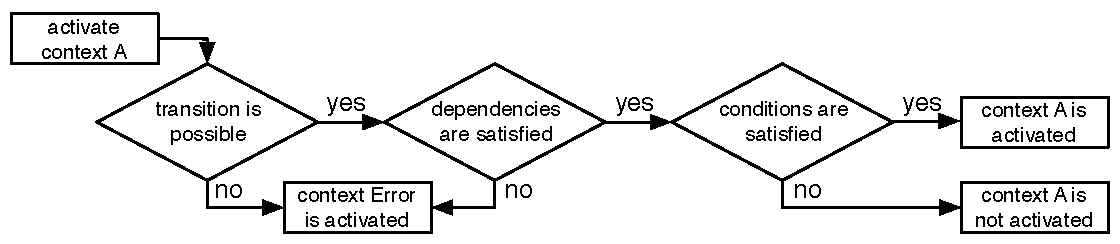
\includegraphics[width=\columnwidth]{pdf/activation_diagram}
}

In our scenario, which is displayed on a figure~\ref{fig:wtd}, within \emph{Activity} group a
transition from \emph{Not Moving} to \emph{Resting} is only possible, and it is checked
by the first conditional chose displayed on a figure~\ref{fig:ad}.
Since each transition is governed by a separate rule, it is declared in a context component as shown
on the line~\lstref{transitions} in figure~\ref{fig:nmc}. Here key-word \emph{transitions}
indicates the contexts a transition can be performed to. An attempt to initiate
a transition to the context, which is not declared in a given active context, leads to an error context
activation, since this kind of transitions is not possible.

\putsnippet{
 caption=NotMoving context.,
 label=fig:nmc,
 boxname=boxnmc
}

Despite the application's  functionality is split into isolated pieces by~\emph{context groups},
there may exist relations among them. For example, within the 
\emph{Base Station} group a transition from \emph{Out Range} to \emph{In Range} is only
make sense if an animal is \emph{Running}. These inter-group relations are covered in our
context-oriented language by context dependencies, which are checked in the second
conditional chose on a figure~\ref{fig:ad}. In ConesC dependencies are declared as
it is shown on the line~\lstref{dependence} in Fig.~\ref{fig:cc}. In \emph{transitions} section a
context name followed by a key-word \emph{iff} and a full name of another context means that
the transition will only be executed if the latter context is active. Should the rule with dependency
be violated, a transition to an error context will be triggered.

The last conditional chose displayed on a figure~\ref{fig:ad} is used for soft rules, violation of
which does not affect the execution of a program. For example, context~\emph{Running} is
activated if the difference between two GPS readings is relatively large, but it may be due to noise.
To make sure false positives are avoided, developers may want to check
readings of an accelerometer. Another example includes energy saving scenario,
when a programmer may want to activate~\emph{In Range} context only if a battery is
in~\emph{Normal} state, as shown in Fig.~\ref{fig:wtd}.
Violation of mentioned rules is a common situation and should not lead to an error state.
To this end, ConesC provides a \emph{check()} command, sample implementation of which is
displayed on the line~\lstref{check} in Fig.~\ref{fig:irc}. It is not mandatory to implement this
command, but should it return \emph{FALSE}, an initiated context transition does not occur,
a context is not activated and a system remains in the previous state.
This approach allows one not to think about conditions a transition taking
place in, but foresee possible inconsistencies.

\putsnippet{
 caption=InRange context.,
 label=fig:irc,
 boxname=boxirc
}

Other types of inter-group relations imply automatic triggering of context
transition. Considering \emph{Battery} group in our example, we can notice that
for further energy saving developers may want to trigger a transition to
\emph{Out Range} context within the \emph{Base Station} group as long as
\emph{Low} context is active. Our design allows one to do that by declaring a
\emph{triggers} section, as shown on the line~\lstref{triggers} in Fig.~\ref{fig:lc}.
The same checks apply to automatic transitions.

\putsnippet{
 caption=Low context.,
 label=fig:lc,
 boxname=boxlc
}
